% ==========================================
% CHAPITRE 2
% ==========================================
\newpage
\chapter{Analyse et planification du projet}
\vspace{2cm}

\noindent \textbf{\Large Plan}
\vspace{1cm}
\begin{enumerate}[label=\textbf{\arabic*}, leftmargin=1.5cm, labelsep=0.8cm]
    \item[] \hspace*{-1.5cm}\textbf{Introduction} \dotfill \pageref{sec:intro_ch2}
    \item \textbf{Identification des acteurs} \dotfill \pageref{sec:acteurs}
    \item \textbf{Spécification des besoins} \dotfill \pageref{sec:besoins}
    \item \textbf{Pilotage du projet avec Scrum} \dotfill \pageref{sec:scrum_pilotage}
    \item \textbf{Backlog du Produit} \dotfill \pageref{sec:backlog}
    \item \textbf{Diagramme de cas d'utilisation global} \dotfill \pageref{sec:use_case}
    \item \textbf{Planification préliminaire des sprints} \dotfill \pageref{sec:planif_sprints}
    \item \textbf{Environnement de travail} \dotfill \pageref{sec:env_tech}
    \item \textbf{Architecture du projet} \dotfill \pageref{sec:architectures}
    \item[] \hspace*{-1.5cm}\textbf{Conclusion} \dotfill \pageref{sec:conclusion_ch2}
\end{enumerate}
\vfill
\newpage

\section*{Introduction}\label{sec:intro_ch2}
Ce chapitre constitue le pivot méthodologique entre la compréhension du contexte projet et la réalisation technique. Il couvre l'intégralité de la phase d'analyse et de planification de PaieZone RH, structurée autour de
quatre axes complémentaires.
Dans un premier temps, nous procédons à l'identification des acteurs du système et à la spécification exhaustive
des besoins fonctionnels et non fonctionnels. Dans un second temps, nous détaillons le pilotage agile du projet :
composition de l'équipe Scrum, construction du Product Backlog de 61 User Stories et planification préliminaire des
quatre sprints. Nous présentons ensuite l'environnement de travail — matériel et logiciel — ayant servi au
développement. Enfin, nous exposons les deux niveaux d'architecture retenus pour la solution : l'architecture
physique de déploiement trois-tiers et l'architecture logique N-tiers conforme aux recommandations JHipster, qui
constituent le cadre technique structurant l'ensemble du développement.
\section{Identification des acteurs}\label{sec:acteurs}
L'identification des acteurs permet de comprendre qui interagit avec le système et quelles sont leurs responsabilités respectives au sein de la solution SaaS.

Conformément au formalisme UML, une relation de généralisation lie les acteurs Admin et RH Comptable : l'acteur
Admin hérite de l'ensemble des droits et fonctionnalités de l'acteur RH Comptable, et dispose en sus de ses propres
prérogatives d'administration

Le tableau \ref{tab:acteurs} présente les différents acteurs du système ainsi que leurs responsabilités respectives.
\renewcommand{\arraystretch}{2.2}

\begin{longtable}{|>{\raggedright\arraybackslash\bfseries}p{3.5cm}|p{\dimexpr\linewidth-3.5cm-4\tabcolsep-2\arrayrulewidth}|}

\hline
\rowcolor[HTML]{EFEFEF}
\textbf{Acteur} & \textbf{Description et responsabilités} \\
\hline
\endfirsthead

\hline
\rowcolor[HTML]{EFEFEF}
\textbf{Acteur} & \textbf{Description et responsabilités} \\
\hline
\endhead
\hline
\endfoot
\hline
\caption{Tableau des acteurs et responsabilités}
\label{tab:acteurs}
\endlastfoot
Visiteur &
\begin{itemize}[label=\tiny\textbullet, nosep, leftmargin=0.4cm]
    \item Accès à la plateforme PaieZone en tant qu'internaute non authentifié.
    \item Soumission du formulaire d'inscription pour l'adhésion au service.
    \item Création simultanée du compte Administrateur et provisionnement de l'espace isolé de l'entreprise (Tenant Provisioning).
    \item Acquisition automatique du rôle Admin Entreprise à l'issue de la démarche d'inscription.
\end{itemize} \\ \hline

Utilisateur \newline (tous rôles) &
\begin{itemize}[label=\tiny\textbullet, nosep, leftmargin=0.4cm]
    \item Authentification sécurisée sur la plateforme PaieZone.
    \item Authentification à double facteur (2FA) obligatoire pour les profils Super Admin et Admin Entreprise.
\end{itemize} \\ \hline

Super Admin &
\begin{itemize}[label=\tiny\textbullet, nosep, leftmargin=0.4cm]
    \item Visualisation et supervision globale des tenants (entreprises clientes).
    \item Gestion des abonnements et des quotas de la plateforme SaaS.
    \item Maintenance globale et supervision technique du système.
    \item Configuration et mise à jour des paramètres réglementaires globaux~\cite{loifinance}.
    \item Gestion et injection automatisée par IA des matrices de conventions collectives sectorielles tunisiennes~\cite{cdt}.
\end{itemize} \\ \hline

Admin Entreprise &
\begin{itemize}[label=\tiny\textbullet, nosep, leftmargin=0.4cm]
    \item Héritage intégral des droits et fonctionnalités du profil RH Comptable.
    \item Gestion des utilisateurs internes et des rôles au sein de l'entreprise.
    \item Consultation et suivi des journaux d'audit de sécurité.
    \item Modification et mise à jour des informations légales de l'entreprise (Raison sociale, identifiant unique).
    \item Invitation de nouveaux collaborateurs sur la plateforme par email.
\end{itemize} \\ \hline

RH Comptable &
\begin{itemize}[label=\tiny\textbullet, nosep, leftmargin=0.4cm]
    \item Configuration et paramétrage de la structure organisationnelle (départements, postes).
    \item Gestion complète des dossiers salariés et des contrats de travail~\cite{cdt}.
    \item Pilotage du cycle complet de la paie et validation finale des bulletins mensuels~\cite{loifinance, cnss_reg}.
    \item Gestion opérationnelle des temps (congés, absences) et traitement des demandes d'avances.
    \item Configuration de l'intégration comptable, génération des écritures et des déclarations réglementaires.
    \item Interaction avec le chatbot IA~\cite{chatbot_hr} pour le support interne et réglementaire.
\end{itemize} \\ \hline

Employé &
\begin{itemize}[label=\tiny\textbullet, nosep, leftmargin=0.4cm]
    \item Consultation de l'espace personnel sécurisé.
    \item Visualisation, consultation et téléchargement des bulletins de paie électroniques.
    \item Soumission et suivi des demandes de congés et d'avances sur salaire.
    \item Interaction avec le chatbot IA~\cite{chatbot_hr} pour l'assistance et les requêtes RH internes.
\end{itemize} \\ 
\end{longtable}
\section{Spécification des besoins}\label{sec:besoins}

Dans cette section, nous allons nous intéresser aux besoins des utilisateurs de notre plateforme en définissant les spécifications fonctionnelles et non fonctionnelles. L'objectif est de concevoir une application performante et adaptée aux attentes du client, afin d'élaborer le Backlog du produit de manière claire et structurée.

\subsection{Besoins fonctionnels}

Les besoins fonctionnels de PaieZone ont été identifiés et organisés par acteur.

Le tableau \ref{tab:besoins-fonctionnels} présente, pour chaque acteur, l'ensemble des fonctionnalités attendues du système.

\renewcommand{\arraystretch}{1.8}

\begin{longtable}{|p{3.5cm}|p{\dimexpr\linewidth-3.5cm-4\tabcolsep-2\arrayrulewidth}|}

\hline
\rowcolor[HTML]{EFEFEF}
\textbf{Acteur} & \textbf{Fonctionnalité} \\ \hline
\endfirsthead

\hline
\rowcolor[HTML]{EFEFEF}
\textbf{Acteur} & \textbf{Fonctionnalité} \\ \hline
\endhead

\hline
\endfoot
\hline
\caption{Tableau des besoins fonctionnels par acteur}
\label{tab:besoins-fonctionnels}
\endlastfoot

% ── Utilisateur ──────────────────────────────────────────
\textbf{Utilisateur} & S'authentifier au système (2FA~\cite{totp} pour comptes sensibles) \\ \hline

% ── Super Admin ──────────────────────────────────────────
{\textbf{Super Admin}}
    & Visualiser et superviser les tenants (entreprises clientes) \\ \cline{2-2}
    & Gérer les entreprises (supprimer, suspendre, réactiver) \\ \cline{2-2}
    & Gérer les abonnements (affecter, modifier) \\ \cline{2-2}
    & Gérer les paramètres réglementaires~\cite{loifinance} (consulter, ajouter, modifier, consulter l'historique) \\ \cline{2-2}
    & Gérer les abonnements (affecter, modifier) \\ \cline{2-2}
    & Gérer le référentiel des conventions sectorielles~\cite{cdt} (consultation, modification et ajout intelligent par IA)\\ \hline

\textbf{Admin Entreprise}
    & Créer et enregistrer une entreprise \\ \cline{2-2}
    & Modifier les informations légales de l'entreprise (raison sociale, identifiant unique) \\ \cline{2-2}
    & Superviser et suivre le type d'abonnement souscrit \\ \cline{2-2}
    & Gérer les utilisateurs internes (créer, modifier, désactiver) \\ \cline{2-2}
    & Consulter et filtrer le journal d'audit \\ \cline{2-2}
    & Gérer la structure organisationnelle (départements, postes) \\ \cline{2-2}
    & Gérer les employés (créer, modifier, désactiver, consulter) \\ \cline{2-2}
    & Gérer les contrats de travail~\cite{cdt} (associer, modifier, résilier) \\ \cline{2-2}
    & Gérer les documents administratifs et légaux \\ \cline{2-2}
    & Gérer les périodes de paie (créer, modifier, clôturer) \\ \cline{2-2}
    & Gérer les rubriques et primes de paie \\ \cline{2-2}
    & Gérer les demandes d'avance (valider, refuser) \\ \cline{2-2}
    & Générer les bulletins de paie~\cite{loifinance} \\ \cline{2-2}
    & Gérer les congés et absences (types, validation, jours fériés) \\ \cline{2-2}
    & Configurer et exporter les données comptables \\ \cline{2-2}
    & Générer les déclarations réglementaires (CNSS~\cite{cnss_reg}, CAVIS, IRPP~\cite{loifinance}) \\ \cline{2-2}
    & Générer les documents officiels (attestation de salaire, certificat de travail) \\ \hline

% ── RH / Comptable ───────────────────────────────────────
\textbf{RH / Comptable}
    & Gérer la structure organisationnelle (départements, postes) \\ \cline{2-2}
    & Gérer les employés (créer, modifier, désactiver, consulter) \\ \cline{2-2}
    & Gérer les contrats de travail~\cite{cdt} (associer, modifier, résilier) \\ \cline{2-2}
    & Gérer les documents administratifs et légaux \\ \cline{2-2}
    & Consulter l'historique des modifications du dossier employé \\ \cline{2-2}
    & Gérer les périodes de paie (créer, modifier, clôturer) \\ \cline{2-2}
    & Gérer les rubriques et primes de paie \\ \cline{2-2}
    & Gérer les demandes d'avance (valider, refuser) \\ \cline{2-2}
    & Générer les bulletins de paie~\cite{loifinance} \\ \cline{2-2}
    & Gérer les congés et absences (types, validation, jours fériés) \\ \cline{2-2}
    & Configurer et exporter les données comptables \\ \cline{2-2}
    & Générer les déclarations réglementaires (CNSS salarié~\cite{cnss_reg}, CNSS employeur~\cite{cnss_reg}, CAVIS, IRPP~\cite{loifinance}) \\ \cline{2-2}
    & Générer les documents officiels (attestation de salaire, certificat de travail) \\ \hline

% ── Employé ──────────────────────────────────────────────
\textbf{Employé}
    & Consulter son espace personnel (profil, informations contractuelles) \\ \cline{2-2}
    & Visualiser et télécharger ses bulletins de paie \\ \cline{2-2}
    & Soumettre et suivre ses demandes de congés \\ \cline{2-2}
    & Consulter son solde de congés \\ \cline{2-2}
    & Soumettre une demande d'avance sur salaire \\ \cline{2-2}
    & Accéder aux services RH via le chatbot intelligent~\cite{chatbot_hr,rag_paper} (questions RH, demandes) \\ \hline

\end{longtable}

\renewcommand{\arraystretch}{1.0}

\subsection{Besoins non fonctionnels}

Au-delà des fonctionnalités métier, la qualité d'une plateforme SaaS repose sur un ensemble de contraintes non fonctionnelles qui conditionnent sa fiabilité, sa sécurité et son acceptabilité par les utilisateurs. Les exigences non fonctionnelles de PaieZone sont les suivantes :

\begin{itemize}[label=\textbullet, leftmargin=*, itemsep=6pt, topsep=6pt, parsep=0pt]
    
    \item \textbf{Sécurité et Confidentialité } La sécurité de PaieZone repose sur plusieurs mécanismes complémentaires : (i)
  l'authentification par tokens JWT à durée de vie limitée, renforcée par une authentification à deux facteurs (TOTP)
  pour les comptes à accès sensible (Super Admin, Admin) ; (ii) le contrôle d'accès basé sur les rôles (RBAC) via
  l'annotation @PreAuthorize de Spring Security, assurant que chaque utilisateur n'accède qu'aux ressources
  autorisées par son profil ; (iii) l'isolation totale des données de chaque entreprise cliente (tenant) via un
  schéma PostgreSQL dédié, rendant toute fuite inter-tenant architecturalement impossible ; (iv) un journal d'audit
  immuable (append-only) enregistrant chaque action sensible avec horodatage, identité de l'auteur, adresse IP et
  valeurs avant/après modification.

    \item \textbf{Réactivité :} L'application Angular~\cite{angular} est une Single Page Application (SPA) bénéficiant d'un design adaptatif. Les temps de réponse des API REST doivent être inférieurs à 2~secondes pour les opérations courantes. Le moteur de calcul de paie doit traiter l'intégralité des bulletins d'une société de 500 employés en moins de 30~secondes.
    
    \item \textbf{Compatibilité :} L'interface utilisateur est conçue pour fonctionner de manière optimale sur les principaux navigateurs modernes (Chrome, Firefox, Edge) et s'adapte automatiquement aux résolutions desktop et tablette, garantissant une accessibilité universelle depuis n'importe quel terminal.
    
    \item \textbf{Extensibilité :} L'architecture modulaire permet d'ajouter des modules ou des types de déclarations sans modifier l'existant. Les taux légaux sont stockés en base de données pour une mise à jour facile et modifiables via l'interface sans redéploiement applicatif, garantissant l'adaptation annuelle aux évolutions de la Loi de Finances tunisienne~\cite{loifinance}.
    
    \item \textbf{Performance :} Le système doit maintenir des temps de réponse acceptables sous charge concurrente, y compris avec
    plusieurs dizaines de tenants actifs simultanément. Le traitement des événements asynchrones (alertes d'expiration
    de contrat, notifications, messages du chatbot) ne doit pas bloquer les transactions métier synchrones. Ces
    exigences sont satisfaites grâce aux choix architecturaux détaillés à la section architecture physique.
    \item \textbf{Maintenabilité :} L'architecture modulaire de \pz\ permet l'ajout de nouveaux modules sans modification de l'existant (principe Open/Closed). Les migrations de schéma sont intégralement gérées par Liquibase de manière versionnée, garantissant la traçabilité et la reproductibilité de tout changement de base de données.
    
    \item \textbf{Portabilité :} L'ensemble des services (backend Spring Boot, base de données PostgreSQL, broker de messages) est conteneurisé via Docker, assurant un déploiement uniforme et reproductible quel que soit l'environnement cible (développement, recette, production).
    
    \item \textbf{Disponibilité :} En tant que solution SaaS, \pz\ est conçue pour une disponibilité continue. Les mises à jour réglementaires (taux CNSS, barèmes IRPP) sont déployées de manière centralisée sans interruption de service pour les tenants actifs.
\end{itemize}


\section{Pilotage du projet avec Scrum}\label{sec:scrum_pilotage}
Le pilotage de PaieZone RH s'inscrit dans le cadre méthodologique Scrum présenté au chapitre 1. Cette section
détaille la composition de l'équipe projet et l'attribution des rôles Scrum, conformément aux pratiques agiles
adoptées.

\subsection{Équipe et rôles Scrum}

Le tableau \ref{tab:equipe_scrum} suivant présente la composition de l'équipe projet et l'attribution des rôles selon le cadre Scrum~\cite{scrum} :

\begin{table}[htbp]
    \centering
    \renewcommand{\arraystretch}{1.8}
    \begin{tabularx}{\textwidth}{|>{\raggedright\arraybackslash\bfseries}p{4.2cm}|>{\raggedright\arraybackslash}p{4cm}|X|}
        \hline
        \rowcolor[HTML]{EFEFEF}
        Rôle Scrum & Membre & Fonction \\ \hline
        Product Owner  & Hadj Amor Ramzi & Directeur technique  (ComptaZone) \\ \hline
        Scrum Master & Hmidi Salim & Encadrant entreprise \newline (Grow Up Technologies) \\ \hline
        Équipe de développement & Chayma Bouguerra \newline Takwa Boughmadi & Étudiante en licence DSI \newline (ISET Mahdia) \\ \hline
    \end{tabularx}
    \caption{Équipe Scrum du projet PaieZone RH}
    \label{tab:equipe_scrum}
\end{table}
% ─────────────────────────────────────────────────────────
\section{Backlog du Produit}\label{sec:backlog}
% ─────────────────────────────────────────────────────────

Le Product Backlog est l'artefact central de la méthode Scrum~\cite{scrum}. Il constitue la liste ordonnée et priorisée de l'ensemble des fonctionnalités et améliorations attendues du produit, et représente la seule source de référence pour tout changement à y apporter. Il est la propriété exclusive du Product Owner, qui en assure la priorisation et le raffinement continu au fil du projet.

Le tableau du Product Backlog s'articule autour des colonnes suivantes, dont la définition garantit une lecture uniforme par toutes les parties prenantes :

\begin{itemize}[label=\textbullet, leftmargin=1.5cm, itemsep=0.5cm]
    \item \textbf{ID :} Identifiant unique de la User Story, permettant de la référencer sans ambiguïté dans le Product Backlog.
    \item \textbf{Épic :} Thème fonctionnel majeur regroupant plusieurs User Stories liées à un même domaine métier.
    \item \textbf{User Story :} Exigence fonctionnelle exprimée du point de vue de l'utilisateur, selon le format canonique : « En tant que [acteur], je veux [action] afin de [bénéfice métier]. »
    \item \textbf{Bénéfice métier :} Valeur attendue par l'utilisateur, exprimée sous la forme « Afin de [valeur métier] ». Les critères d'acceptation détaillés et les règles techniques sont précisés dans les backlogs de sprint correspondants (Chapitres 3 à 6).
    \item \textbf{Sprint :} Itération de développement au cours de laquelle la User Story est planifiée et réalisée. Les estimations en jours-homme associées sont détaillées dans les backlogs de sprint respectifs.
    \item \textbf{Priorité :} Niveau d'importance de la User Story pour la réussite du produit, déterminé par le Product Owner selon la valeur métier et les dépendances techniques. Quatre niveaux sont définis : Critique, Haute, Moyenne, Faible.
\end{itemize}

Le tableau~\ref{tab:backlog} présente le Product Backlog complet, organisé par épics et user stories.

\renewcommand{\arraystretch}{1.8}

\renewcommand{\arraystretch}{1.8}

\begin{xltabular}{\textwidth}{|>{\centering\arraybackslash}p{0.8cm}|>{\raggedright\arraybackslash}p{3.2cm}|>{\raggedright\arraybackslash}X|>{\raggedright\arraybackslash}X|>{\centering\arraybackslash}p{1.6cm}|}
\hline
\rowcolor[HTML]{EFEFEF}
\textbf{ID} & \textbf{Épic} & \textbf{User Story} & \textbf{Bénéfice métier} & \textbf{Priorité} \\
\hline
\endfirsthead

\hline
\rowcolor[HTML]{EFEFEF}
\textbf{ID} & \textbf{Épic} & \textbf{User Story} & \textbf{Bénéfice métier} & \textbf{Priorité} \\
\hline
\endhead

\hline
\endfoot

\caption{Product Backlog complet de PaieZone RH}
\label{tab:backlog}
\endlastfoot

% ── Épic 1 ───────────────────────────────────────────────
1 & Gestion de l'authentification et des accès
  & En tant qu'utilisateur, je veux m'authentifier~\cite{jwt}
  & Afin d'accéder au système de manière sécurisée
  & Critique \\ \hline

% ── Épic 2 ───────────────────────────────────────────────
2 & \multirow{6}{3.2cm}{Gestion des entreprises}
  & En tant qu'Admin, je veux créer une entreprise
  & Afin de l'enregistrer dans le système
  & Critique \\ \cline{3-5}
  & & En tant qu'Admin, je veux modifier une entreprise
  & Afin de mettre à jour ses informations
  & Haute \\ \cline{3-5}
  & & En tant qu'Admin, je veux désactiver une entreprise
  & Afin de suspendre son accès
  & Haute \\ \cline{3-5}
  & & En tant que Super Admin, je veux affecter un abonnement
  & Afin de gérer les droits d'accès
  & Critique \\ \cline{3-5}
  & & En tant que Super Admin, je veux modifier un abonnement
  & Afin de changer le plan souscrit
  & Moyenne \\ \cline{3-5}
  & & En tant que Super Admin, je veux résilier un abonnement
  & Afin d'arrêter le service
  & Moyenne \\ \hline

% ── Épic 3 ───────────────────────────────────────────────
3 & \multirow{3}{3.2cm}{Gestion des utilisateurs et des habilitations}
  & En tant qu'Admin, je veux créer un utilisateur
  & Afin de lui donner un accès (RBAC~\cite{rbac})
  & Critique \\ \cline{3-5}
  & & En tant qu'Admin, je veux modifier un utilisateur
  & Afin de mettre à jour ses données et ses accès
  & Haute \\ \cline{3-5}
  & & En tant qu'Admin, je veux désactiver un utilisateur
  & Afin de retirer son accès
  & Haute \\ \hline

% ── Épic 4 ───────────────────────────────────────────────
4 & \multirow{2}{3.2cm}{Traçabilité et journal d'audit}
  & En tant qu'Admin, je veux consulter le journal d'audit
  & Afin de voir les actions effectuées
  & Haute \\ \cline{3-5}
  & & En tant qu'Admin, je veux filtrer le journal d'audit
  & Afin de rechercher des actions spécifiques
  & Moyenne \\ \hline

% ── Épic 5 ───────────────────────────────────────────────
5 & \multirow{6}{3.2cm}{Gestion de la structure organisationnelle}
  & En tant qu'Admin/RH, je veux créer un département
  & Afin de structurer l'entreprise
  & Haute \\ \cline{3-5}
  & & En tant qu'Admin/RH, je veux modifier un département
  & Afin de mettre à jour la structure
  & Haute \\ \cline{3-5}
  & & En tant qu'Admin/RH, je veux désactiver un département
  & Afin de le retirer de la structure
  & Moyenne \\ \cline{3-5}
  & & En tant qu'Admin/RH, je veux créer un poste
  & Afin de définir un rôle
  & Haute \\ \cline{3-5}
  & & En tant qu'Admin/RH, je veux modifier un poste
  & Afin de l'adapter aux besoins
  & Moyenne \\ \cline{3-5}
  & & En tant qu'Admin/RH, je veux désactiver un poste
  & Afin de le retirer de la structure
  & Moyenne \\ \hline

% ── Épic 6 ───────────────────────────────────────────────
6 & \multirow{5}{3.2cm}{Gestion du capital humain}
  & En tant qu'Admin/RH, je veux consulter la liste des employés
  & Afin d'avoir une vue d'ensemble du personnel
  & Haute \\ \cline{3-5}
  & & En tant qu'Admin/RH, je veux créer un employé
  & Afin de l'ajouter au système
  & Critique \\ \cline{3-5}
  & & En tant qu'Admin/RH, je veux consulter le profil d'un employé
  & Afin de voir ses informations détaillées
  & Haute \\ \cline{3-5}
  & & En tant qu'Admin/RH, je veux modifier un employé
  & Afin de mettre à jour ses données
  & Haute \\ \cline{3-5}
  & & En tant qu'Admin/RH, je veux désactiver un employé
  & Afin de gérer sa sortie de l'organisation
  & Haute \\ \hline

% ── Épic 7 ───────────────────────────────────────────────
7 & \multirow{3}{3.2cm}{Gestion du cycle de vie des contrats de travail}
  & En tant que RH, je veux associer un contrat à un employé~\cite{cdt}
  & Afin de formaliser la relation de travail
  & Critique \\ \cline{3-5}
  & & En tant que RH, je veux modifier un contrat
  & Afin de changer ses conditions
  & Haute \\ \cline{3-5}
  & & En tant que RH, je veux résilier un contrat
  & Afin de terminer une relation de travail
  & Haute \\ \hline

% ── Épic 8 ───────────────────────────────────────────────
8 & Gestion des documents administratifs et légaux
  & En tant que RH, je veux déposer un document
  & Afin de le stocker dans le dossier employé
  & Moyenne \\ \hline

% ── Épic 9 ───────────────────────────────────────────────
9 & Historisation et suivi
  & En tant qu'Admin/RH, je veux consulter l'historique des modifications
  & Afin de tracer les changements du dossier employé
  & Haute \\ \hline

% ── Épic 10 ──────────────────────────────────────────────
10 & \multirow{4}{3.2cm}{Gestion des paramètres réglementaires}
   & En tant que Super Admin, je veux consulter la liste des paramètres réglementaires~\cite{loifinance}
   & Afin de vérifier les taux légaux en vigueur
   & Haute \\ \cline{3-5}
   & & En tant que Super Admin, je veux ajouter un nouveau paramètre réglementaire
   & Afin d'intégrer une nouvelle règle légale
   & Haute \\ \cline{3-5}
   & & En tant que Super Admin, je veux modifier un paramètre réglementaire
   & Afin de mettre à jour les taux conformément à la loi
   & Haute \\ \cline{3-5}
   & & En tant que Super Admin, je veux consulter l'historique des modifications des paramètres
   & Afin de garantir la traçabilité réglementaire
   & Moyenne \\ \hline

% ── Épic 11 ──────────────────────────────────────────────
11 & \multirow{13}{3.2cm}{Gestion de la paie}
   & En tant que RH, je veux créer une période de paie
   & Afin de lancer le cycle de traitement des salaires
   & Critique \\ \cline{3-5}
   & & En tant que RH, je veux modifier une période de paie
   & Afin de corriger les données avant clôture
   & Haute \\ \cline{3-5}
   & & En tant que RH, je veux clôturer une période de paie
   & Afin de valider et verrouiller les calculs
   & Critique \\ \cline{3-5}
   & & En tant que RH, je veux lancer le calcul de tous les bulletins d'une période
   & Afin de générer automatiquement les salaires nets~\cite{loifinance}
   & Critique \\ \cline{3-5}
   & & En tant que RH, je veux créer une rubrique de paie
   & Afin de structurer les éléments de calcul
   & Haute \\ \cline{3-5}
   & & En tant que RH, je veux modifier une rubrique de paie
   & Afin de l'adapter aux besoins de la société
   & Moyenne \\ \cline{3-5}
   & & En tant que RH, je veux ajouter une prime à un employé
   & Afin d'augmenter sa rémunération pour une période
   & Haute \\ \cline{3-5}
   & & En tant que RH, je veux modifier une prime
   & Afin d'ajuster son montant avant le calcul
   & Moyenne \\ \cline{3-5}
   & & En tant que RH, je veux valider une demande d'avance
   & Afin d'accorder le soutien financier sollicité
   & Haute \\ \cline{3-5}
   & & En tant que RH, je veux refuser une demande d'avance
   & Afin d'informer l'employé du rejet de sa demande
   & Haute \\ \cline{3-5}
   & & En tant qu'employé, je veux demander une avance sur salaire
   & Afin de recevoir un soutien financier ponctuel
   & Haute \\ \cline{3-5}
   & & En tant que RH, je veux générer un bulletin de paie
   & Afin de le distribuer à l'employé concerné
   & Critique \\ \cline{3-5}
   & & En tant que RH, je veux générer un fichier CNSS~\cite{cnss_reg}
   & Afin de déclarer les salariés auprès de la CNSS
   & Critique \\ \hline

% ── Épic 12 ──────────────────────────────────────────────
12 & \multirow{5}{3.2cm}{Gestion des congés et des absences}
   & En tant que RH, je veux créer un type de congé
   & Afin de définir les règles et quotas associés
   & Haute \\ \cline{3-5}
   & & En tant qu'employé, je veux demander un congé
   & Afin de m'absenter légitimement
   & Haute \\ \cline{3-5}
   & & En tant que RH, je veux valider une demande de congé
   & Afin de gérer la disponibilité de l'équipe
   & Haute \\ \cline{3-5}
   & & En tant qu'employé, je veux consulter mon solde de congé
   & Afin de planifier mes absences
   & Haute \\ \cline{3-5}
   & & En tant que RH, je veux gérer les jours fériés
   & Afin de les intégrer dans le calcul de paie~\cite{loifinance}
   & Moyenne \\ \hline

% ── Épic 13 ──────────────────────────────────────────────
13 & \multirow{2}{3.2cm}{Intégration comptable et finance RH}
   & En tant qu'Admin/RH, je veux configurer le plan comptable
   & Afin de structurer la comptabilité de la société
   & Haute \\ \cline{3-5}
   & & En tant qu'Admin/RH, je veux exporter les données comptables au format SAGE
   & Afin de les synchroniser avec le logiciel comptable
   & Haute \\ \hline

% ── Épic 14 ──────────────────────────────────────────────
14 & \multirow{4}{3.2cm}{Conformité et déclarations réglementaires}
   & En tant que RH, je veux générer une déclaration CNSS salarié~\cite{cnss_reg}
   & Afin de respecter les obligations légales
   & Critique \\ \cline{3-5}
   & & En tant que RH, je veux générer une déclaration CNSS employeur~\cite{cnss_reg}
   & Afin de respecter les obligations légales
   & Critique \\ \cline{3-5}
   & & En tant que RH, je veux générer une déclaration CAVIS~\cite{cnss_reg}
   & Afin de satisfaire aux obligations réglementaires
   & Haute \\ \cline{3-5}
   & & En tant que RH, je veux générer une déclaration IRPP~\cite{loifinance}
   & Afin de déclarer les retenues à la source
   & Critique \\ \hline

% ── Épic 15 ──────────────────────────────────────────────
15 & \multirow{2}{3.2cm}{Génération des documents officiels RH}
   & En tant que RH, je veux générer une attestation de salaire
   & Afin de justifier les revenus d'un employé
   & Haute \\ \cline{3-5}
   & & En tant que RH, je veux générer un certificat de travail~\cite{cdt}
   & Afin d'attester de la relation contractuelle
   & Haute \\ \hline

% ── Épic 16 ──────────────────────────────────────────────
16 & \multirow{3}{3.2cm}{Assistant RH intelligent (Chatbot)}
   & En tant qu'utilisateur, je veux accéder à un assistant conversationnel RH~\cite{chatbot_hr}
   & Afin d'obtenir des réponses rapides à mes questions administratives
   & Moyenne \\ \cline{3-5}
   & & En tant qu'employé, je veux demander un congé via le chatbot
   & Afin de simplifier la soumission de ma demande
   & Moyenne \\ \cline{3-5}
   & & En tant qu'employé, je veux consulter mon bulletin via le chatbot~\cite{rag_paper}
   & Afin d'y accéder rapidement sans navigation manuelle
   & Moyenne \\ \hline

\end{xltabular}
\renewcommand{\arraystretch}{1.0}
% ─────────────────────────────────────────────────────────
\section{Diagramme de cas d'utilisation global}\label{sec:use_case}
% ─────────────────────────────────────────────────────────
Le diagramme de cas d’utilisation global offre une synthèse structurée des interactions entre les divers acteurs et le système. Il permet d'appréhender de manière globale le périmètre fonctionnel de la solution. 

La Figure \ref{fig:use_case_global} expose ce diagramme, mettant en exergue les relations clés entre les utilisateurs et les fonctionnalités majeures de la plateforme.

\begin{figure}[h!]
    \centering
    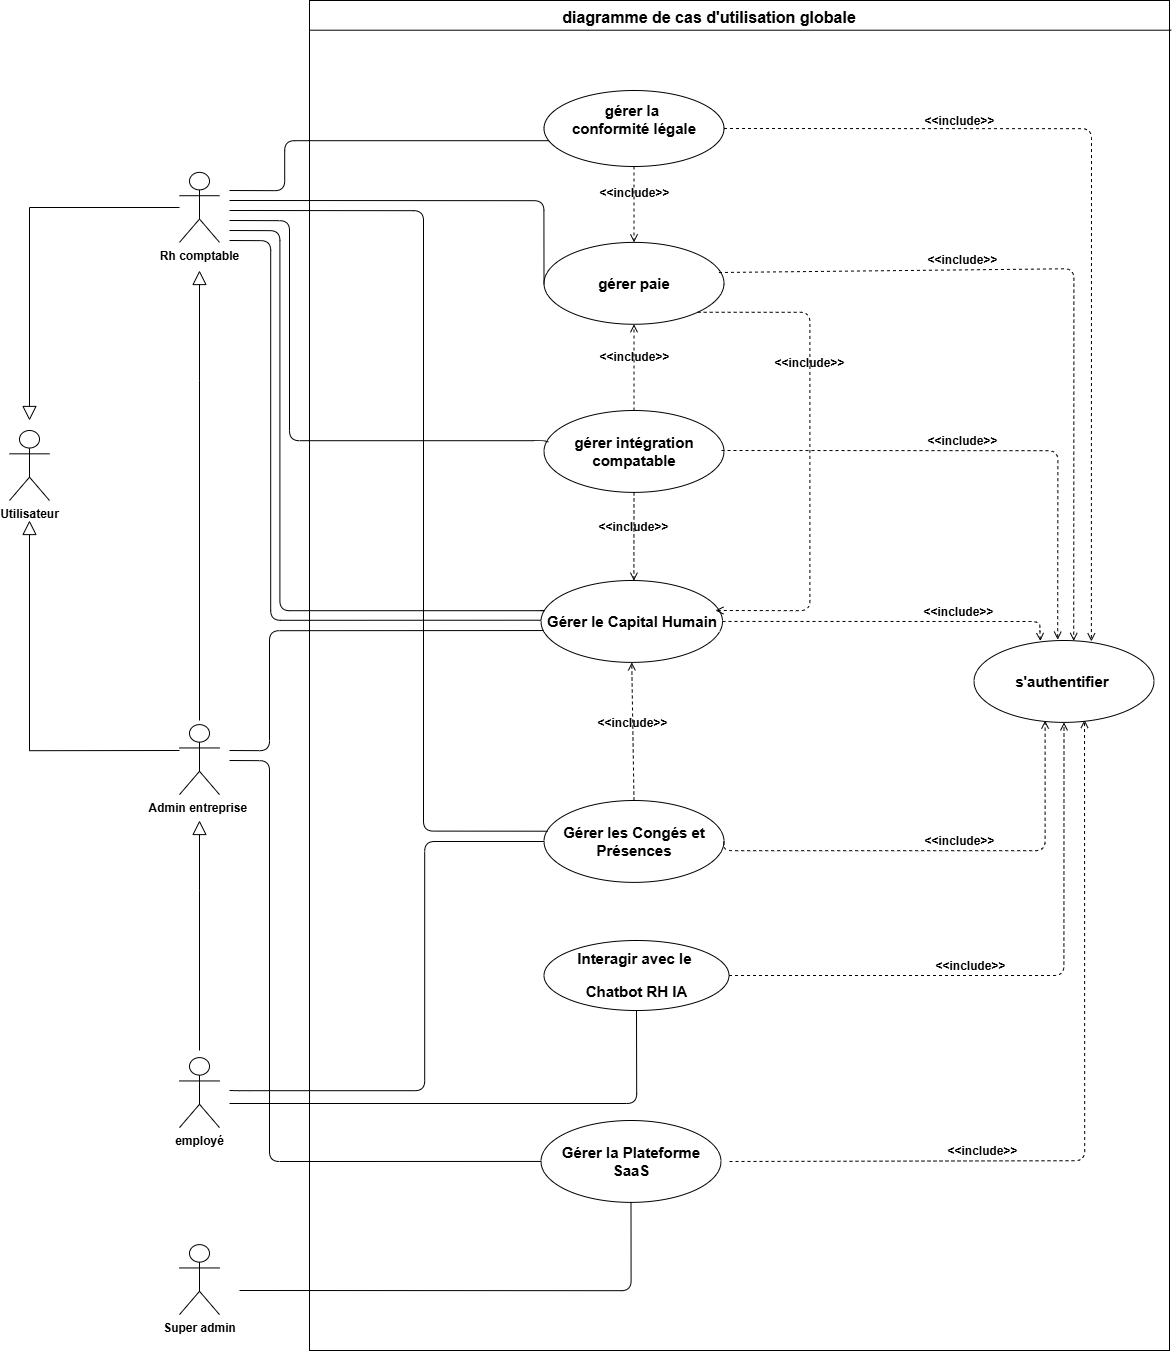
\includegraphics[width=0.9\textwidth]{diagramme-globale-F.png}
    \caption{Diagramme de cas d'utilisation global de PaieZone RH}
    \label{fig:use_case_global}
\end{figure}
\newpage

% ─────────────────────────────────────────────────────────
\section{Planification préliminaire des sprints}\label{sec:planif_sprints}
% ─────────────────────────────────────────────────────────
La planification des sprints a été établie en tenant compte de deux contraintes majeures : les dépendances techniques entre les modules et la valeur métier livrable à chaque itération. Le projet est découpé en 4 sprints de 3 semaines chacun conformément aux recommandations de Scrum~\cite{scrum}.
\newpage
\begin{table}[h]
    \centering
    \renewcommand{\arraystretch}{1.8}
    \begin{tabularx}{\textwidth}{|>{\raggedright\arraybackslash\bfseries}p{4.5cm}|X|}
        \hline
        \rowcolor[HTML]{EFEFEF}
        Sprint / Itération & Objectifs et Fonctionnalités \\ \hline
        \vspace{0.5cm}\centering
        
\includegraphics[width=2.5cm, valign=m]{sprint1.png} \par
        \textbf{Socle \& Sécurité}  &
        \begin{itemize}[label=--, nosep, leftmargin=0.4cm] \setstretch{1.6}
            \item Authentification (JWT~\cite{jwt})
            \item Inscription des entreprises
            \item Gestion des rôles et permissions (RBAC~\cite{rbac})
            \item Approbation du compte utilisateur (2FA~\cite{totp})
            \item Gestion du profil utilisateur
            \item Gestion des départements et postes
        \end{itemize} \\ \hline
        \vspace{0.1cm}\centering
        
\includegraphics[width=2.5cm, valign=m]{sprint 2.png}\par
        \textbf{Gestion Administrative} &
        \setstretch{1.6}
        \begin{itemize}[label=--, nosep, leftmargin=0.4cm]
            \item Création et suivi des dossiers employés
            \item Gestion des contrats de travail~\cite{cdt}
            \item Alertes d'expiration de contrats
            \item Historique des modifications
        \end{itemize} \\ \hline
        \vspace{0.2cm}\centering
        
\includegraphics[width=2.5cm, valign=m]{sprint 3.png}\par
        \textbf{Paie \& Congés}   &
        \begin{itemize}[label=--, nosep, leftmargin=0.4cm] \setstretch{1.6}
            \item Calcul automatique de la paie~\cite{loifinance}
            \item Gestion des congés et absences
            \item Génération des bulletins de paie
            \item Workflow de validation des congés
        \end{itemize} \\ \hline
        \vspace{0.2cm}\centering
        
\includegraphics[width=2.5cm, valign=m]{sprint 4.png} \par
        \textbf{Conformité \& IA} &
        \begin{itemize}[label=--, nosep, leftmargin=0.4cm] \setstretch{1.6}
            \item Déclarations sociales (CNSS~\cite{cnss_reg}, IRPP~\cite{loifinance})
            \item Génération des écritures comptables
            \item Chatbot RH intelligent~\cite{rag_paper,chatbot_hr}
            \item Recommandations et assistance intelligente
        \end{itemize} \\ \hline
    \end{tabularx}
    \caption{Tableau de planification préliminaire des sprints}
\end{table}
\vspace{1cm}

% ─────────────────────────────────────────────────────────
\section{Environnement de travail}\label{sec:env_tech}
% ─────────────────────────────────────────────────────────
Cette section présente l'environnement global dans lequel le projet a été conçu, développé et testé. 

Elle détaille d'une part l'infrastructure matérielle utilisée pour supporter la charge de calcul, et d'autre part l'écosystème logiciel et technique ayant servi à l'implémentation de la solution.

\subsection{Environnement matériel}
Le choix de l'architecture matérielle est une étape cruciale pour garantir la fluidité des cycles de compilation, la virtualisation des services de données et l'exécution locale des modules d'intelligence artificielle. Les ressources physiques mobilisées se répartissent sur les postes de travail décrits ci-dessous.
\subsubsection{Poste de travail n°1}
Le tableau \ref{tab:pc_chayma_final} détaille les caractéristiques techniques du premier poste de travail :

\begin{table}[htbp]
    \centering
    \renewcommand{\arraystretch}{1.5}
    \begin{tabular}{|>{\raggedright\arraybackslash\bfseries}p{5cm}|>{\raggedright\arraybackslash}p{4.9cm}|}
        \hline
        \rowcolor[HTML]{EFEFEF}
        Composant & Spécification \\ \hline
        Marque & ASUS TUF Gaming F15 \\ \hline
        Processeur & Intel Core i7-13620H \\ \hline
        Mémoire RAM & 16 Go DDR4 \\ \hline
        Disque dur & SSD NVMe 512 Go \\ \hline
        Système d'exploitation & Windows 11 Famille \\ \hline
        \multicolumn{2}{|c|}{
            \begin{minipage}{9.9cm}
                \centering
                \vspace{0.1cm}
                
\includegraphics[height=2.5cm]{pc_chayma}
                \vspace{0.1cm}
            \end{minipage}
        } \\ \hline
    \end{tabular}
    \caption{Caractéristiques matérielles et aperçu du poste n°1}
    \label{tab:pc_chayma_final}
\end{table}

\subsubsection{Poste de travail n°2}
Le tableau \ref{tab:pc_takwa_final} détaille les caractéristiques techniques du second poste de travail :
\newpage
\begingroup
\renewcommand{\arraystretch}{1.5}
\begin{longtable}{|>{\raggedright\arraybackslash\bfseries}p{4.8cm}|>{\raggedright\arraybackslash}p{5.1cm}|}

   \hline
    \rowcolor[HTML]{EFEFEF}
    Composant & Spécification \\
    \hline
    \endfirsthead

    \endhead
    \footnotetext{}
    \endfoot
    \endfoot

    %% ── PIED DERNIÈRE PAGE ──
    \hline
    \caption{Caractéristiques matérielles et aperçu du poste n°2}
    \label{tab:pc_takwa_final}
    \endlastfoot

    Marque               & ASUS VivoBook X515EP  \\ \hline
    Processeur           & Intel Core i5-1135G7  \\ \hline
    Mémoire RAM          & 16 Go                 \\ \hline
    Disque dur           & SSD NVMe 512 Go       \\ \hline
    Système d'exploitation & Windows 11 Famille  \\ \hline

    \multicolumn{2}{|c|}{%
        \begin{minipage}{9.9cm}
            \centering
            \vspace{0.2cm}
            
\includegraphics[height=2.5cm]{pc_takwa}
            \vspace{0.2cm}
        \end{minipage}
    } \\ \hline

\end{longtable}
\endgroup
\subsection{Environnement logiciel}

Le tableau \ref{tab:tools_logos_final} recense l'ensemble des outils et technologies utilisés pour le développement de la plateforme \pz{} :

\begingroup
\renewcommand{\arraystretch}{1.5}
% Largeur totale augmentée à 13.7 cm (parfait pour remplir l'espace de la page sans déborder)
\begin{longtable}{|>{\raggedright\arraybackslash\bfseries}p{3.2cm}|>{\raggedright\arraybackslash}p{7.5cm}|>{\centering\arraybackslash}m{3.0cm}|}
    \hline
    \rowcolor[HTML]{EFEFEF}
    Outil \& Version & Description et rôle & Logo \\
    \hline
    \endfirsthead

    \endhead
    \footnotetext{}
    \endfoot
    \endfoot

    %% ── PIED DERNIÈRE PAGE ──
    \hline
    \caption{Environnement logiciel, outils et technologies du projet}
    \label{tab:tools_logos_final}
    \endlastfoot

    JHipster 9.x~\cite{jhipster} & Générateur Full-stack utilisé pour le squelette applicatif, la sécurité JWT et les migrations Liquibase~\cite{liquibase}. & 
\includegraphics[height=1cm]{logo_jhipster} \\ \hline
    Angular 18.x~\cite{angular} & Framework frontend pour la SPA. Utilisation des \textit{signals} et de l'internationalisation FR/AR. & 
\includegraphics[height=0.9cm]{logo_angular} \\ \hline
    Spring Boot 4.0~\cite{springboot} & Backend REST sécurisé (JWT~\cite{jwt} + RBAC~\cite{rbac}). Gestion de l'audit et de l'envoi d'emails. & 
\includegraphics[height=1.2cm]{logo_springboot.png} \\ \hline
    PostgreSQL 15.x~\cite{postgresql} & Base de données relationnelle. Isolation multi-tenant~\cite{multitenant} via un schéma dédié par entreprise. & 
\includegraphics[height=1cm]{logo_postegre.png} \\ \hline
    Ollama \& Phi-3 & Environnement d'exécution de modèles de langage en local (LLM). Le modèle open-source Phi-3 (Microsoft) est exploité pour propulser le Chatbot RH intelligent, garantissant la confidentialité des données de paie sans dépendance à des API tierces payantes. & 
\includegraphics[height=1cm]{ollama.png} \\ \hline
    IntelliJ IDEA & Environnement de développement intégré (IDE) principal pour le backend Spring Boot/Java. & 
\includegraphics[height=0.9cm]{logo_intellij} \\ \hline
    GitHub & Plateforme de gestion de versions et de collaboration pour le contrôle des sources. & 
\includegraphics[height=0.9cm]{logo_github.png} \\ \hline
    Draw.io & Outil de diagrammatique en ligne utilisé pour la conception des diagrammes UML~\cite{uml} et d'architecture. & 
\includegraphics[height=0.9cm]{logo draw.png} \\ \hline
    Google Meet & Outil de visioconférence utilisé pour les réunions d'équipe et les sprints reviews. & 
\includegraphics[height=0.9cm]{google meet.png} \\ \hline
    Google Chat & Messagerie instantanée d'équipe pour les communications quotidiennes et le partage de ressources. & 
\includegraphics[height=0.9cm]{logo_intellij} \\ \hline
    Docker 24.x & Conteneurisation de tous les services pour un déploiement unifié (backend, base de données, Kafka~\cite{kafka}). & 
\includegraphics[height=1cm]{logo_docker} \\ \hline
    Lucidchart & Outil de modélisation visuelle utilisé en complément pour la conception des diagrammes de flux. & 
\includegraphics[height=0.9cm]{logo lucid.png} \\ \hline
    \LaTeX & Système de composition typographique utilisé pour la rédaction du présent rapport de PFE. & 
\includegraphics[height=0.7cm]{logo_latex.png} \\ \hline

\end{longtable}
\endgroup
% ─────────────────────────────────────────────────────────
\section{Architecture du projet}\label{sec:architectures}
% ─────────────────────────────────────────────────────────
L'architecture d'un système logiciel définit l'organisation structurelle de ses composants 
et les principes régissant leurs interactions. Pour PaieZone, deux niveaux d'architecture 
ont été définis : une architecture physique qui décrit l'organisation des composants matériels 
et réseau, et une architecture logique qui précise la structure interne du code et les couches 
applicatives.

% ── 2.8.1 ──────────────────────────────────────────────
\subsection{Architecture physique (déploiement)}
L'architecture physique de PaieZone, conforme aux principes du Cloud Computing~\cite{saas}, 
s'appuie sur un modèle trois-tiers classique, organisé en trois couches distinctes et 
indépendantes :

\begin{itemize}[label=\textbullet, leftmargin=*, itemsep=6pt, topsep=6pt, parsep=0pt]
    \item \textbf{Couche Client (Tier 1) :} Navigateurs web des utilisateurs finaux (Chrome, 
    Firefox, Edge) accédant à l'interface Angular~\cite{angular} via HTTPS. L'application est 
    une SPA : après le chargement initial, toutes les interactions avec le serveur transitent 
    par des appels API REST asynchrones (sans rechargement de page), garantissant une expérience 
    utilisateur fluide.

    \item \textbf{Couche Serveur Applicatif (Tier 2) :} Serveur hébergeant le backend Spring 
    Boot~\cite{springboot} (JAR exécutable dans un conteneur Docker). Il expose une API REST 
    documentée via Swagger/OpenAPI~3, sécurisée par tokens JWT~\cite{jwt}. Ce niveau intègre 
    également un cache applicatif assuré par Caffeine (cache en mémoire JVM) pour les données 
    fréquemment accédées (listes de tenants, paramètres réglementaires), garantissant des temps 
    de réponse optimaux sans dépendance externe, ainsi qu'Apache Kafka~\cite{kafka} comme broker 
    de messages pour le traitement asynchrone des événements non bloquants : alertes d'expiration 
    de contrats CDD, notifications de validation de congés et de demandes d'avance. Ce découplage 
    garantit la fluidité de l'application principale même sous forte charge multi-tenant.

    \item \textbf{Couche Persistance (Tier 3) :} Serveur PostgreSQL~15~\cite{postgresql}, 
    organisé en schémas multiples : un schéma public pour les données de gouvernance SaaS 
    (tenants~\cite{multitenant}, abonnements, Super Admin) et un schéma dédié 
    (ex : \texttt{tn\_acme\_sa}) pour les données métier de chaque entreprise cliente. 
    Liquibase~\cite{liquibase} assure les migrations de schéma de manière versionnée.
\end{itemize}

\begin{figure}[ht!]
    \centering
    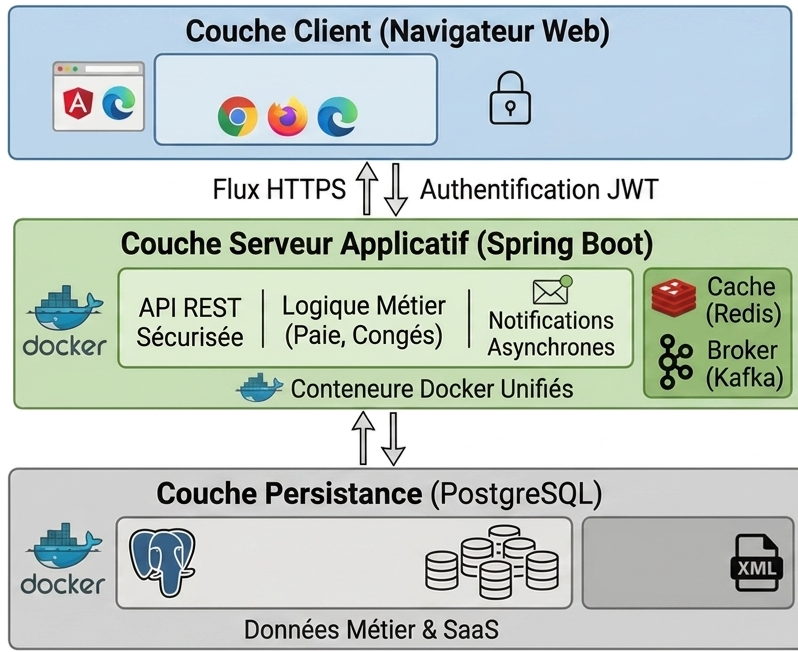
\includegraphics[width=0.87\textwidth]{architecture_logique.png}
    \caption{Architecture physique trois-tiers}
    \label{fig:architecture_physique}
\end{figure}

% ── 2.8.2 ──────────────────────────────────────────────
\subsection{Architecture logique du système}
PaieZone est développé selon une architecture N-tiers (architecture en couches), conforme 
aux recommandations JHipster~\cite{jhipster} et aux bonnes pratiques du développement Spring 
Boot~\cite{springboot}. Cette architecture s'articule autour de cinq couches verticales, 
traversées par deux couches transversales.

La figure ~\ref{fig:architecture_logique} présente les différentes couches de l'architecture 
logique du système ainsi que leurs rôles respectifs.

\begin{itemize}[label=\textbullet, leftmargin=*, itemsep=6pt, topsep=6pt, parsep=0pt]

    \item \textbf{Couche Présentation (Web Layer) :} Assurée par les contrôleurs REST Spring 
    Boot~\cite{springboot} (\texttt{@RestController}), elle expose les endpoints HTTP sous le 
    préfixe \texttt{/api/pz/}. Elle gère la validation (\texttt{@Valid}), la sérialisation 
    JSON (Jackson) et la pagination.

    \item \textbf{Couche Service (Business Layer) :} Cœur de la logique métier (annotée 
    \texttt{@Service}). Elle contient les règles de calcul de paie (Loi de Finances 
    2026~\cite{loifinance}), les workflows d'approbation et la logique 
    multi-tenant~\cite{multitenant}. La cohérence est garantie par \texttt{@Transactional}.

    \item \textbf{Couche Accès aux Données (Repository Layer) :} Implémentée via Spring Data 
    JPA et les repositories étendant \texttt{JpaRepository}. L'isolation multi-tenant est 
    assurée par un mécanisme en deux niveaux : (i) le \texttt{TenantContextService} extrait 
    l'identifiant du tenant depuis le token JWT~\cite{jwt} à chaque requête ; (ii) le 
    \texttt{DatabaseConfiguration} applique dynamiquement la commande 
    \texttt{SET search\_path TO <schema\_tenant>, public} sur la connexion 
    PostgreSQL~\cite{postgresql}, redirigeant toutes les requêtes JPA vers le schéma isolé 
    de l'entreprise concernée. Cette approche garantit qu'aucune requête ne peut accéder aux 
    données d'un autre tenant, même en cas de bug applicatif.

    \item \textbf{Couche Modèle (Domain Layer) :} Contient les entités JPA 
    (\textit{Employee, Contract, Payslip, etc.}) et les DTO assurant le découplage entre 
    persistance et présentation.

    \item \textbf{Couches transversales :} La \textbf{Sécurité} (Spring 
    Security~\cite{springboot}) valide les tokens JWT~\cite{jwt} et les rôles 
    RBAC~\cite{rbac} (\texttt{@PreAuthorize}), tandis que l'\textbf{Audit} (Spring AOP) 
    enregistre toutes les écritures dans un journal immuable.
\end{itemize}

\begin{figure}[ht!]
    \centering
    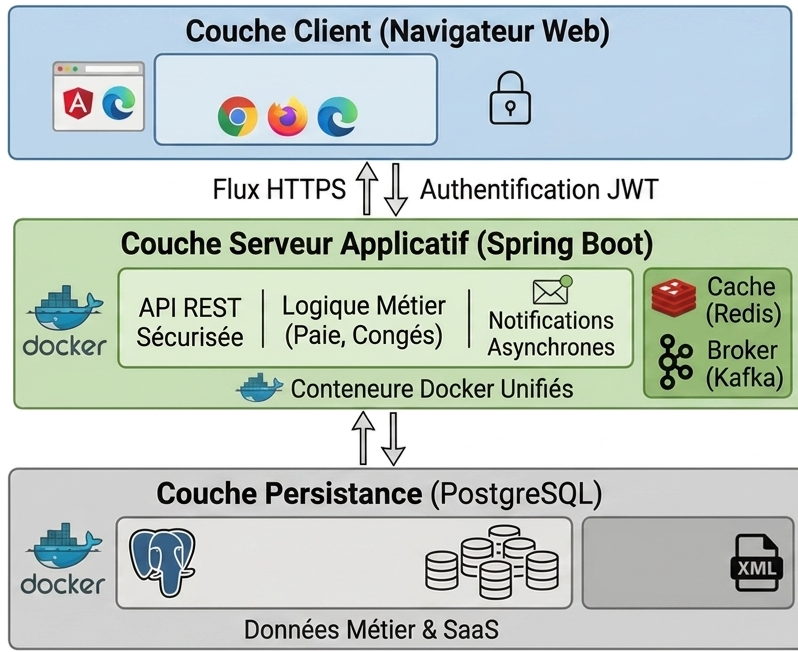
\includegraphics[width=0.85\textwidth]{architecture_logique.png}
    \caption{Architecture logique N-tiers (Spring Boot / Angular)}
    \label{fig:architecture_logique}
\end{figure}
\vfill
\newpage

% ── Conclusion ─────────────────────────────────────────
\section*{Conclusion}\label{sec:conclusion_ch2}
Ce chapitre a posé les fondements analytiques et méthodologiques du projet PaieZone RH. Nous avons défini cinq
 acteurs aux responsabilités distinctes — Visiteur, Super Admin, Admin Entreprise, RH Comptable et Employé — et
 formalisé leurs besoins à travers un Product Backlog structuré de 61 User Stories, réparties en seize épics
 fonctionnels. Les exigences non fonctionnelles identifiées — sécurité, confidentialité, performance,
 maintenabilité, portabilité et disponibilité — constituent les critères de qualité transversaux que chaque sprint
 devra respecter. L'architecture N-tiers adoptée, conforme aux recommandations JHipster, offre une séparation claire
 des responsabilités et un mécanisme multi-tenant robuste basé sur l'isolation par schéma PostgreSQL. Les choix
 technologiques retenus — Spring Boot 4.0, Angular 18, PostgreSQL 15, Kafka et Ollama — positionnent PaieZone comme
 une solution SaaS moderne, performante et évolutive. Fort de ces fondations, le chapitre suivant présente les
 travaux du premier sprint, consacré à l'implémentation du socle de sécurité, de la gestion multi-tenant et de la
 traçabilité par journal d'audit.
